\documentclass[twocolumn]{article}

\usepackage[margin=0.75in]{geometry}
\usepackage{amsmath}
\usepackage{amssymb}
\usepackage{graphicx}
\usepackage{hyperref}
\usepackage{cite}

\title{\textbf{Thermodynamic Cloaking of Inward Civilizations:\\Evolutionary Dynamics and Observational Constraints from the Far-Infrared Gap}}
\author{\textbf{Satoshi Yamashita} \\ \small Independent Researcher, Tokyo, Japan}
\date{\today}

\begin{document}
\maketitle

\begin{abstract}
The Fermi Paradox traditionally presupposes macroscopic, Kardashev-style expansion. However, physical communication latencies and entropy limits favor dimensionally condensed, inward computation. Using a spatial Moran process on a 2D galactic torus, we demonstrate that macro-expansionist clades fail to percolate ($R_0 < 1$), whereas inward-computational clades achieve a silent dynamic equilibrium ($f_{\mathrm{intro}} \approx 14\%$). Coupling this equilibrium with Landauer thermodynamics for extreme capacities ($\dot{I} \sim 10^{40}\ \mathrm{bits\ s^{-1}}$), we show that optimal cryogenic dissipation ($T_{\mathrm{rad}} \sim 10\text{--}30\ \mathrm{K}$) shifts emissions directly into the Far-Infrared Gap ($30\text{--}300\ \mu\mathrm{m}$). This signature evaded Herschel and remains marginally below ALMA, yet is resolvable via the submillimeter spectral index ($\alpha \approx 2.0$ vs. $\beta \approx 1.7$ dust). Comparisons with COBE/FIRAS confirm this population satisfies galactic background limits, framing the Great Silence as a consequence of thermodynamic optimization.
\end{abstract}

\section{Introduction}
The absence of detectable signatures from extraterrestrial intelligences, formalized as the Fermi Paradox, has spurred hypotheses ranging from rare abiogenesis to civilizational self-destruction. A persistent assumption underlying classical formulations is the inevitability of outward physical colonization. Here, we analyze whether physical constraints dictate an inward evolutionary transition.

\section{Galactic Evolutionary Dynamics}
To assess civilizational competition over astronomical epochs, we formalize a spatial Moran process over a discrete torus. The effective reproduction number $R_0$ of outward expansion is given by:
\begin{equation}
R_0 = \frac{p_{\mathrm{expand}} (1 - s_{\mathrm{travel}}) P(\mathrm{Empty})}{\mathrm{decay}_{\mathrm{extrovert}} + s_{\mathrm{purge}} P(\mathrm{Contact})}
\end{equation}

\begin{figure}[htbp]
\centering
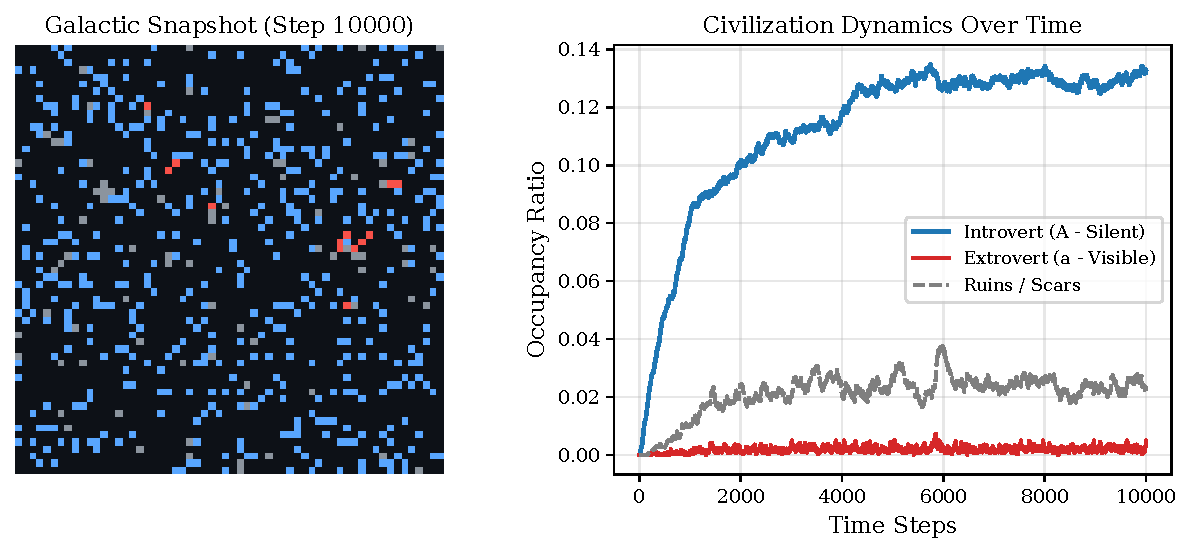
\includegraphics[width=\columnwidth]{../figures/fig1_dynamics.pdf}
\caption{Galactic snapshot and long-term population frequency over 10,000 steps ($f_{\mathrm{intro}} \approx 14\%$).}
\label{fig:dynamics}
\end{figure}

\section{Thermodynamic Dissipation and Spectroscopic Constraints}
Any information-processing architecture is fundamentally bounded by Landauer's principle:
\begin{equation}
P_{\mathrm{waste}} \ge \dot{I} k_B T_{\mathrm{rad}} \ln 2
\end{equation}
Assuming optimal heat rejection via blackbody radiator geometry:
\begin{equation}
A_{\mathrm{rad}} = \frac{\dot{I} k_B \ln 2}{\epsilon \sigma T_{\mathrm{rad}}^3}
\end{equation}

\begin{figure}[htbp]
\centering
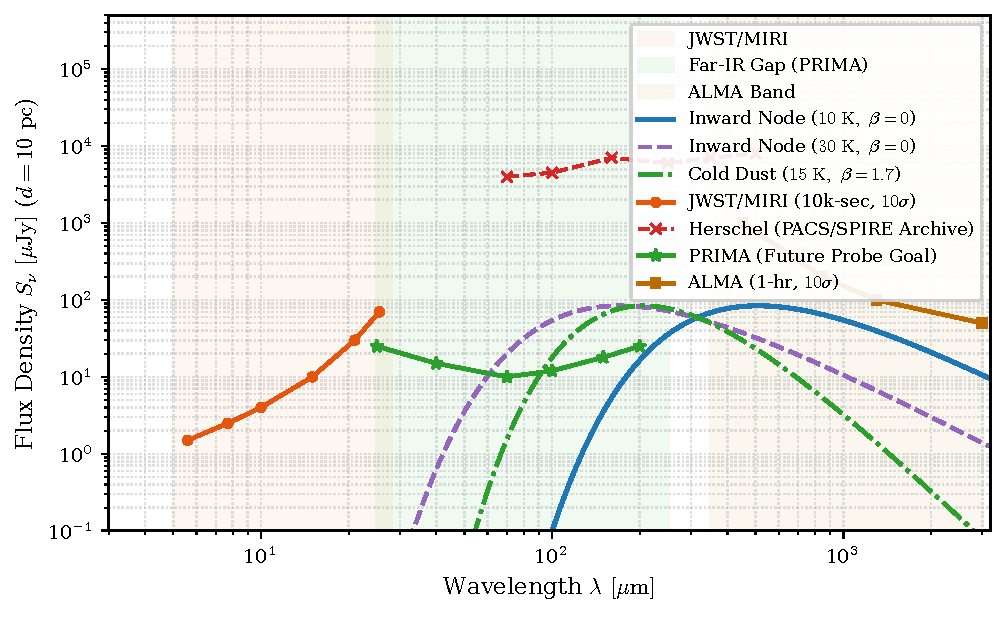
\includegraphics[width=\columnwidth]{../figures/fig2_spectra.pdf}
\caption{Observed spectral flux density for an inward node at $d = 10\ \mathrm{pc}$ contrasted with telescope sensitivities and natural cold dust.}
\label{fig:spectra}
\end{figure}

\section{Galactic Background Constraints}
Integrating over the total stellar population of the Milky Way ($N_\star \approx 10^{11}$):
\begin{equation}
L_{\mathrm{total}} = f_{\mathrm{intro}} N_\star (\dot{I} k_B T_{\mathrm{rad}} \ln 2)
\end{equation}

\begin{figure}[htbp]
\centering
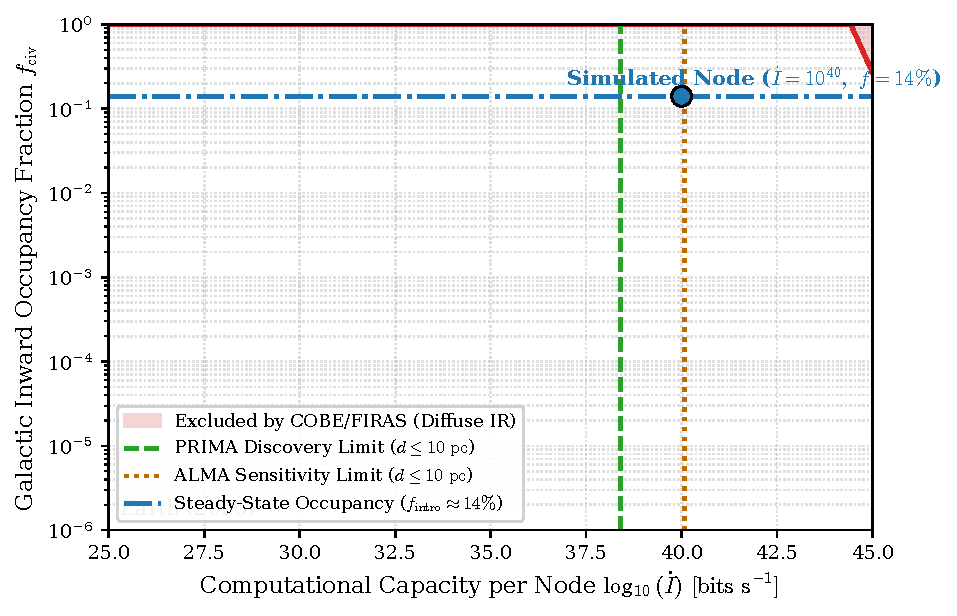
\includegraphics[width=\columnwidth]{../figures/fig3_exclusion.pdf}
\caption{Parameter exclusion plot constrained by COBE/FIRAS diffuse background observations.}
\label{fig:exclusion}
\end{figure}

\section{Discussion and Conclusion}
The transition from unconstrained expansion to inward optimization directly resolves the Great Silence. Forthcoming missions such as PRIMA will directly test the identified parameter regime.

\bibliographystyle{plain}
\bibliography{references}

\end{document}
